\documentclass[11pt]{article}

\usepackage{pablo}
\usepackage[a5paper,margin=1.2cm]{geometry}
\usepackage{enumerate}

\usepackage{multicol}

\pagestyle{empty}
\begin{document}

\begin{center}
  {\large
    Devoir surveillé
    ---
    \textsc{Vecteurs}
  }

  Correction
\end{center}

\begin{em}
  \noindent Les questions originales sont en italique.
\end{em}


\begin{exercice}[Relation de Chasles --- 3 points] \emph{Exprimer le plus
  simplement possible les sommes de vecteurs suivants :}
  \begin{multicols}{2}
    \begin{enumerate}[(a)]
      \item $\vecteur{AB}+\vecteur{BC} = \vecteur{AC}$
      \item $\vecteur{EF}+\vecteur{AE}-\vecteur{AF}$\\
        $= \vecteur{AE}+\vecteur{EF} + \vecteur{FA}$ \\
        $= \vecteur{AA} = \vecteur{0}$
      \columnbreak
      \item $\vecteur{AB}+\vecteur{CA}-\vecteur{DB}-\vecteur{CD}$\\
        $= \vecteur{AB} + \vecteur{CA} + \vecteur{BD} + \vecteur{DC}$\\
        $= \vecteur{AB} + \vecteur{BD} + \vecteur{DC} + \vecteur{CA}$\\
        $= \vecteur{AA} = \vecteur{0}$
      \item $2\vecteur{DB}+\vecteur{BD}-\vecteur{AB}$\\
        $= \vecteur{DB} + \vecteur{DB} + \vecteur{BD} + \vecteur{BA}$\\
        $= \vecteur{DB} + \vecteur{BA} = \vecteur{DA}$
    \end{enumerate}
  \end{multicols}
\end{exercice}

\begin{exercice}[2 points]
  \emph{Exprimer les vecteur $\vecteur u$ et $\vecteur v$ en fonction des vecteurs
  $\vecteur a$ et $\vecteur b$}.

  \begin{multicols}{2}
    \begin{enumerate}[(a)]
      \item $\vecteur{u}=3\vecteur{a}+\vecteur{b}$

        \tikzstyle{vecteur}=[thick]
        \begin{tikzpicture}[baseline=(current bounding box.north),scale=0.7]
          \draw[thin,color=gray,step=1] (-1,-1) grid (3,4);
          \draw[vecteur,->] (0,0) -- (2,0);
          \draw[vecteur,->] (0,0) -- (0,1);
          \draw[vecteur,->] (0,0) -- (2,3);
          \draw (0,0.5) node[left] {$\vecteur{a}$};
          \draw (1.5,0) node[below] {$\vecteur{b}$};
          \draw (1.5,1.5) node[] {$\vecteur{u}$};

          \draw[vecteur,->,dashed] (0,1) -- (0,2);
          \draw[vecteur,->,dashed] (0,2) -- (0,3);
          \draw[vecteur,->,dashed] (0,3) -- (2,3);
          \draw (0,1.5) node[left] {$\vecteur{a}$};
          \draw (0,2.5) node[left] {$\vecteur{a}$};
          \draw (1.5,3) node[above] {$\vecteur{b}$};
        \end{tikzpicture}

      \item $\vecteur{v} = -2\vecteur{a} + \frac{5}{2}\vecteur{b}$

        \begin{tikzpicture}[baseline=(current bounding box.north),scale=0.7]
          \draw[thin,color=gray,step=1] (-1,-3) grid (6,2);
          \draw[vecteur,->] (0,0) -- (2,0);
          \draw[vecteur,->] (0,0) -- (0,1);
          \draw[vecteur,->] (0,0) -- (5,-2);
          \draw (0,0.5) node[left] {$\vecteur{a}$};
          \draw (1.5,0) node[above] {$\vecteur{b}$};
          \draw (3.5,-0.5) node[] {$\vecteur{v}$};

          \draw[vecteur,dashed,->] (0,0) -- (0,-1);
          \draw[vecteur,dashed,->] (0,-1) -- (0,-2);
          \draw[vecteur,dashed,->] (0,-2) -- (2,-2);
          \draw[vecteur,dashed,->] (2,-2) -- (4,-2);
          \draw[vecteur,dashed,->] (4,-2) -- (5,-2);
          \draw (0,-0.5) node[left] {$\vecteur{-a}$};
          \draw (0,-1.5) node[left] {$\vecteur{-a}$};
          \draw (1,-2) node[below] {$\vecteur{b}$};
          \draw (3,-2) node[below] {$\vecteur{b}$};
          \draw (4.5,-2) node[below] {$\frac{1}{2}\vecteur{b}$};
        \end{tikzpicture}
    \end{enumerate}
  \end{multicols}

\end{exercice}

\begin{exercice}[5 points]
  \emph{Soit $ABCD$ un quadrilatère quelconque, et $I$, $J$, $K$, $L$ les milieux respectifs des segments $[AB]$, $[BC]$, $[CD]$, et $[DA]$.}
  \begin{enumerate}[(a)]
    \item \emph{Sur une figure, placer quatre points $A$, $B$, $C$ et $D$ au
      hasard, et placer les points $I$, $J$, $K$ et $L$ en fonction de $A$,
      $B$, $C$ et $D$. Tracer les quadrilatères $ABCD$ et $IJKL$, et le
      segment $AC$.}

      \begin{center}
        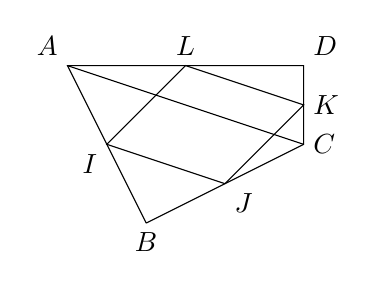
\begin{tikzpicture}[scale=1]
          \draw[-] (-1,0) -- (1,1) -- (1,2) -- (-2,2) -- (-1,0);
          \draw[-] (0,0.5) -- (1,1.5) -- (-0.5,2) -- (-1.5,1) -- (0,0.5);
          \draw[-] (1,1) -- (-2,2);
          \draw (-2,2) node[above left] {$A$};
          \draw (-1,0) node[below] {$B$};
          \draw (1,1) node[right] {$C$};
          \draw (1,2) node[above right] {$D$};
          \draw (-1.5,1) node[below left] {$I$};
          \draw (0,0.5) node[below right] {$J$};
          \draw (1,1.5) node[right] {$K$};
          \draw (-0.5,2) node[above] {$L$};
        \end{tikzpicture}
      \end{center}
      \item \emph{Le but de cette question est de prouver que $\vecteur{IJ}=\frac{1}{2}\vecteur{AC}$.}
        \begin{enumerate}[(i)]
          \item \emph{Justifier que $\vecteur{IJ} = \vecteur{IB}+\vecteur{BJ}$.}

            C'est la relation de Chasles.
          \item \emph{Justifier que $\vecteur{IB}=\vecteur{AI}$ et $\vecteur{BJ}=\vecteur{JC}$.}

            $I$ étant par définition le milieu de $[AB]$, on a $\vecteur{IA}=\vecteur{BI}$. De même pour $J$, milieu de $[BC]$.
          \item \emph{En déduire que $\vecteur{AI}+\vecteur{JC}=\vecteur{IJ}$.}

          La question (i) donne l'égalité $\vecteur{IJ} = \vecteur{IB}+\vecteur{BJ}$. Donc, puisque $\vecteur{IB}=\vecteur{AI}$ et $\vecteur{BJ}=\vecteur{JC}$, on a $\vecteur{AI}+\vecteur{JC}=\vecteur{IJ}$.
          \item \emph{Justifier que $\vecteur{AC}=\vecteur{AI}+\vecteur{IJ}+\vecteur{JC}$.}

            C'est encore une fois l'égalité de Chasles.
          \item \emph{En déduire que $\vecteur{IJ}=\frac{1}{2}\vecteur{AC}$.}

            $\vecteur{AC}=\vecteur{AI}+\vecteur{IJ}+\vecteur{JC} = \vecteur{AI}+\vecteur{JC}+\vecteur{IJ}$

            Or, par (iii), $\vecteur{AI}+\vecteur{JC}=\vecteur{IJ},$ donc :
            $\vecteur{AC}=\vecteur{IJ}+\vecteur{IJ}$.

            Ainsi $\vecteur{AC}=2\vecteur{IJ}$, c'est-à-dire $\frac{1}{2}\vecteur{AC}=\vecteur{IJ}$.
        \end{enumerate}
    \item \emph{En utilisant le même raisonnement, montrer que $\vecteur{LK}=\frac{1}{2}\vecteur{AC}$.}
      Par la relation de Chasles, $\vecteur{LK}=\vecteur{LD}+\vecteur{DK}$. Or, $L$ et $K$ étant respectivement les milieux de $[AD]$ et $[DC]$, $\vecteur{AL}=\vecteur{LD}$ et $\vecteur{DK}=\vecteur{KC}$, donc $\vecteur{LK}=\vecteur{AL}+\vecteur{KC}$.

      Toujours par la relation de Chasles, $\vecteur{AC}=\vecteur{AL}+\vecteur{LK}\vecteur{KC}$, donc $\vecteur{AC}=2\vecteur{LK}$, et $\vecteur{LK}=\frac{1}{2}\vecteur{AC}$.
    \item \emph{En déduire la nature du quadrilatère $IJKL$.}

      Par les questions précédentes, $\vecteur{LK}=\frac{1}{2}\vecteur{AC}=\vecteur{IJ}$, donc $\vecteur{LK}=\vecteur{IJ}$. Donc $IJKL$ est un parallélogramme.
  \end{enumerate}
\end{exercice}

\end{document}
